\section{Design}
\label{sec:design}
%We assume that the underlying network is Ethernet, on which we implemented our
%prototype.

\OurSys infers failing links and follows a policy on how to process
frames that are about to cross failing links. It uses a \emph{forward
error-correction} (FEC) scheme to enable the next hop to recover frames that
were lost in transit by using extra parity frames that are inserted
into the medium.

In this section we describe \OurSys's policy choices for managing failing
links, and how the chosen policy is followed in the network.


\subsection{Traffic classification}
\label{sec:traffic-classification}
\OurSys is configured to have a number of traffic classes,
which partition %s -- # agreement "classes partition"
 the frames arriving at a switch. Outbound frames are encapsulated and
complemented with parity frames, forming \emph{blocks} that are sent across
the faulty link.
Each class $c$ is defined by a map $T: c \mapsto (k, h, t)$, where $k$ is the
number of frames in a block, $h$ is the number of parity frames sent for each
block, and $t$ is the timeout.
%(When the encoding timer expires, the remaining frame spaces in a block are
%zeroed out to provide padding.)
The values $(k, h, t)$ influence the latency with which frames belonging to $c$
cross the switch, as well the likely recovery of frames belonging to $c$.
%For example, for interactive applications we would want to use a
%small $k$ and $t$.

%\lei{Deleted some. Seems to be redundance of 3.3-sending proxy}
%\iffalse
%Parity frames are new frames that are put onto the medium, so by
%increasing $h$ we create more contention for the link, which reduces
%the capacity available for data from applications crossing that link.
%\fi

\subsection{Link-failure management policy}
\label{sec:policy}
For each port the policy stipulates how to react if the link becomes
faulty: frames are either dropped (i.e., the link is disabled), or they are
processed to use FEC.
%  \begin{itemize}
%    \item Drop frames (i.e., disable the link); or
%    \item Classify the frame, encode it, and forward.
%  \end{itemize}
For the latter case, the policy specifies what are the traffic classifications,
and how each classification maps into parameters $(k, h, t)$.
%
%In principle both the map $T$ (from~\S\ref{sec:traffic-classification}) and
%the policy can be decided or changed while \OurSys is running, but for
%consistency not while \OurSys is actually processing frames. In practice it is
%resource-efficient to engineer to a limited set of choices to support.


\subsection{Execution}
\OurSys consists of three concurrent activities carried out for each port of a
switch:
\begin{itemize}
  \item \textbf{Link monitoring agent} attempts to infer link malfunction.
  \item \textbf{Sending proxy} processes frames and adds tags before they are sent over a faulty link.
  \item \textbf{Receiving proxy} processes inbound \OurSys-tagged frames.
\end{itemize}

Frames to be sent over non-faulty links, and inbound frames that are not
\OurSys-tagged, are processed as normal by the switch. Otherwise outgoing frames
are processed by the Sending proxy prior to egress, and inbound frames by
the Receiving proxy after ingress.

\paragraph{Link monitoring agent.}
  We continuously poll network port counters to infer malfunctioning transceiver
  modules or links. This is done as in
  CorrOpt~\cite{Zhuo:2017:UMP:3098822.3098849}, but failure-inference is done
  locally on the switch, rather than remotely.
  Sometimes a switch cannot itself realize if one of its links is
  malfunctioning, since the malfunction would be inferable from the adjacent
  element's counters (e.g., through an increase in frame errors). Thus switches
  might need to inform each other about errors on the transmitting side. To do
  this we employ LLDP and use a custom TLV to signal to the receiving switch
  that the link (for traffic travelling in the opposite direction) is failing.
%  The switch's monitoring would then follow the policy to disable the link, or
%  channel outgoing frames through the Sending proxy.

\paragraph{\OurSys frame encapsulation}
As Fig.~\ref{fig:example-loss} demonstrates, frames sent over faulty links are tagged to allow the receiving switch to distinguish frames processed by \OurSys and to provide the traffic classification and index of a packet within a block. The tag also includes a block identifier to protect against bursty losses.
%\FIXME{Combine Fig.~\ref{fig:example-loss} and Fig.~\ref{fig:example-loss2}, and reference the combined figure here.}

\begin{figure}
  \centering
  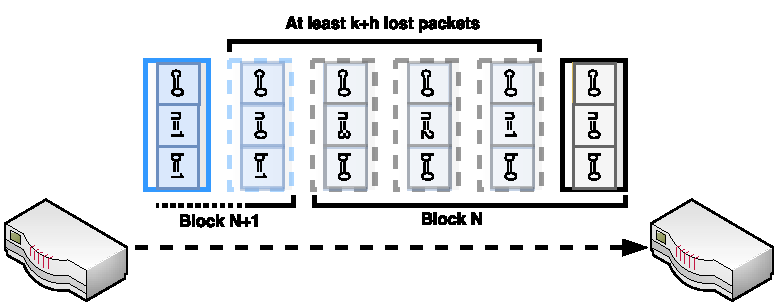
\includegraphics[width=0.35\paperwidth]{figures/example-loss.pdf}
  \caption{\label{fig:example-loss}Packet numbering on lossy link between two switches.  For low failure
  rates, assigning monotonically increasing frame numbers $n$ that are unique within a
  block is sufficient to distinguish successive blocks.  
  On links with bursty loss behavior, adding
  a block sequence number helps to distinguish packets.
% The expectation for strictly monotonic frame
% number $n$ ensures that we can distinguish successive blocks.
  Note that frame
  reordering is not possible because the frames are being sent over the same link,
  and their processing is sequential across that link.}
% \hg{S1 and S2 are not referring to anything anymore as we removed the first figure.}
\end{figure}

\iffalse
\begin{figure}
  \centering
  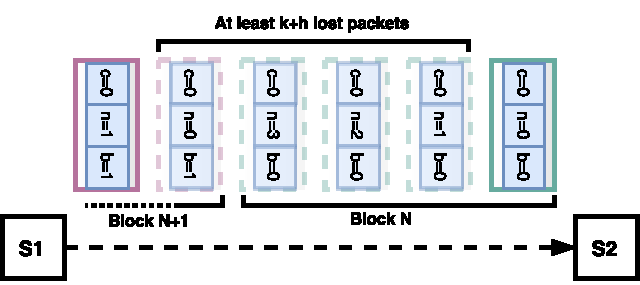
\includegraphics[width=0.35\paperwidth]{figures/paper-fig-5.pdf}
  \caption{\label{fig:example-loss2}On links with bursty loss behavior, adding
           a block sequence number helps to distinguish packets.}
%To mitigate bursty loss, a block sequence number is added.}
% \hg{S1 and S2 are not referring to anything anymore as we removed the first figure.}
\end{figure}
\fi

\paragraph{Sending proxy.}
%The pseudo-code is shown in Algorithm~\ref{alg:sending}.
The encoding of a block -- to produce parity frames -- is
triggered when the block is full (all $k$ frames have been accounted for) or
$t$ for that $c$ expires (relative to when the first frame was inserted into
the block). Non-parity frames are tagged and forwarded immediately.

Due to its operation, the sending proxy can cause congestion at egress.
For example, if $k = h$, and we are receiving traffic bound for
a faulty link at rate $R$, then we would need to send at rate $2R$ at each interval
of $k$ incoming frames, at which time the sending proxy produces $h$ additional
frames for output. We simply drop new frames that cannot be put onto the link
fast enough (i.e., before they are placed into a block).
%This lack of capacity
%is communicated by the $\mathit{busy}(c)$ predicate in
%Algorithm~\ref{alg:sending}, which indicates that the FEC computation is
%ongoing, or its results are still being serialized onto the medium.
This loss will communicate to higher-layer protocols that congestion
is occurring %(both due to the link capacity being reduced, and
%because of the extra overhead of sending the parity frames),
so the
end-hosts' network stacks can react to this congestion as they
normally would.

%\begin{algorithm}
%\SetAlgoLined
%\SetKwInOut{Input}{input}\SetKwInOut{Output}{output}
%\Input{frame to be forwarded}
%\Output{forwarding decision}
%\uIf(\tcc*[h]{Link has been disabled}){policy = drop}{
%drop frame\;
%}\Else(\tcc*[h]{Use FEC}){
%  $c = P(\mathrm{frame})$ \tcc*[l]{Classify the frame}
%  \uIf(\tcc*[h]{Block is being sent}){busy(c)}{
%drop frame\;
%}\Else{
%  $\overline{\mathrm{frame}}$ = encapsulate($c, \mathrm{frame}$)\;
%  addToBlock($c$, $\overline{\mathrm{frame}}$)\;
%  forward $\overline{\mathrm{frame}}$\;
%}
%}
%\caption{\label{alg:sending}Sending proxy. If the block's $k$ has been reached, then addToBlock will start the process of generating and sending parity frames. This process is also begun if the block's $k$ has not been reached but $t$ expires.}
%\hg{The bar above "frame" is confusing.
%    Are you proposing to immediately drop a frame if we happen to be sending
%    another frame?  It would be better to put it in a buffer such that we
%    can send it later.  If the channel remains occupied and the buffer fills
%    up, we can still drop a frame.  The sending of parity frames appears to
%    be somewhere hidden in the algorithm.  The drop policy seems so obvious
%    that I would not even mention it.  Finally, the caption
%    appears to tell a whole algorithm by itself, which makes me wonder why it
%    is not part of the algorithm.}
%\end{algorithm}

\paragraph{Receiving proxy.}
\OurSys-tagged frames are buffered as shown in Fig.~\ref{fig:example-decode},
and non-parity frames are untagged and forwarded immediately.
For each $c$, if its $t$ (relative to when the first
frame was buffered) expires, or a frame from a successive block arrives, 
then decoding is triggered. Decoding consists of using the parity frames to
reconstruct the lost data frames; if no data frames have been lost then there
is no more work to be done for this block.
%\amd{I've been assuming a simpler version...as soon as there are enough
%  packets to perform decoding, we do.  Then we discard any subsequent
%  packets that arrive in the block.  No timeout on decode.  On the FPGA
%  where we are designed for full rate when decoding, this doesn't slow
%  anything down.  On a processor that cannot maintain full-rate decoding,
%  not doing decoding could be a performance optimization.}\\
%\lei{I've switched paragraph 1 and 2, 3 and 4. This order follows the listing at the beginning,
%looks more natural to me, and avoids use-before-define. I also lifted the diagrams. It is difficult
%to understand the design from plain text for people unfamiliar with this. Also, there are too many
%details in caption of diagrams.}

%\begin{algorithm}
%\SetAlgoLined
%\SetKwFunction{FName}{addToBlock}%
%\SetKwProg{Proc}{Procedure}{\string:}{}
%\Proc{\FName{c, frame}}{
%\uIf(\tcc*[h]{Link has been disabled}){policy = drop}{
%drop frame
%}\Else(\tcc*[h]{Use FEC}){
%  $c = P(\mathrm{frame})$\;
%  addToBlock($c$, frame)\;
%}
%}
%\caption{\label{alg:sending}Adding a frame to a block for class $c$}
%\end{algorithm}
\begin{figure}
  \centering
  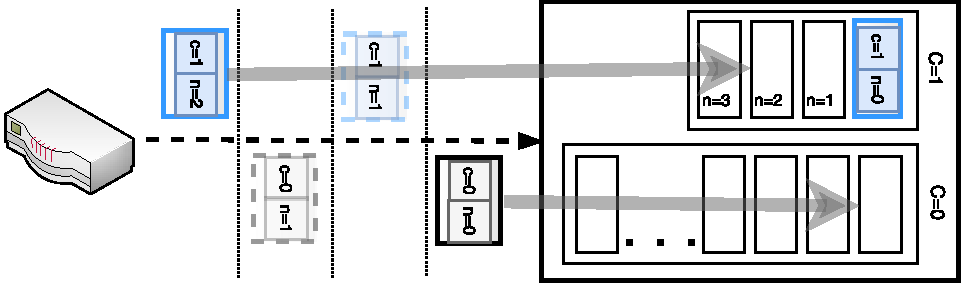
\includegraphics[width=0.4\paperwidth]{figures/example-decode.pdf}
  \caption{\label{fig:example-decode}Prior to decoding a block on arrival, each block is mapped to the buffer for its traffic class. A dotted border indicates that a frame has been lost while transiting.}
\end{figure}
